\providecommand{\HomA}{\mathrm{Hom}_{A}}
\providecommand{\HomB}{\mathrm{Hom}_{B}}
\providecommand{\HomC}{\mathrm{Hom}_{C}}
\providecommand{\colim}{\mathop{\mathrm{colim}}\nolimits}
\providecommand{\ran}{\mathop{\mathrm{ran}}\nolimits}
\providecommand{\lan}{\mathop{\mathrm{lan}}\nolimits}

\section{∞-范畴中的\trWeightedLimit{}与\trWeightedColimit{}}\label{sec:weighted-limits-and-colimits-in-infinity-categories}

在本节中，我们把由定义 9.4.7 所编码的诸\trInfinityCategory{}之间图表的\trLimit{}与%
\trColimit{}推广为由一支\trModule{}加权的\trLimit{}与\trColimit%
。\trWeightedLimit{}与\trWeightedColimit{}的概念涵盖了定义 9.4.7（见%
\cref{ex:ordinary-limits-as-weighted}），而且从模的\trVirtualEquipment{}的观点来看
是相当自然的。
这可以理解为 A.6 节中在\trEnrichedCategory{}的语境下所引入理论的∞-范畴式版本，不过
从一开始，我们就允许诸\textbf{权}（weight）取为\textbf{\trProfunctor}（profunctor），如练习
A.6.iv 中那样。

\begin{definition}\label{def:weighted-limits-colimits}
给定一支\trModule{} $A\xrightarrow{W}B$ 与一个\trFunctor{} $f\colon A\to C$，一个函子
$\lim_{W}f\colon B\to C$ 定义 $f$ 的\textbf{$W$-\trWeightedLimit}，若它共变地表示
$\HomC(C,f)$ 沿 $W$ 的右\trExtension{}。对偶地，给定 $A\xrightarrow{W}B$ 与一个%
\trFunctor{} $g\colon B\to C$，一个函子 $\colim_{W}g\colon A\to C$ 定义 $g$ 的%
\textbf{$W$-\trWeightedColimit}，若它反变地表示 $\HomC(g,C)$ 穿过 $W$ 的右\trLifting{}。
\begin{center}
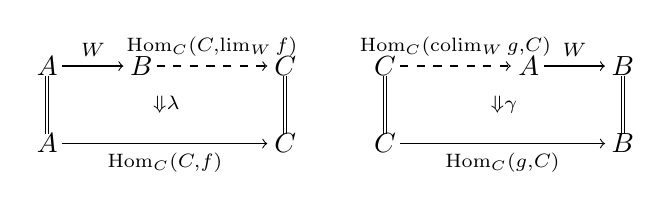
\begin{tikzpicture}[x=1.0em,y=1.0em]
  \begin{scope}
    \node at (0,1.4)   {$A$};
    \node at (3.4,1.4) {$B$};
    \node at (8.6,1.4) {$C$};
    \draw[->] (0.55,1.4) -- node[above]{$\scriptstyle W$} (2.75,1.4);
    \draw[->,dashed] (3.95,1.4) -- node[above]{$\scriptstyle\HomC(C,\lim_{W}f)$} (7.95,1.4);
    \draw[double,double distance=0.6pt] (0,1.05) -- (0,-1.05);
    \draw[double,double distance=0.6pt] (8.6,1.05) -- (8.6,-1.05);
    \node at (4.3,0) {$\scriptstyle\Downarrow\lambda$};
    \node at (0,-1.4)   {$A$};
    \node at (8.6,-1.4) {$C$};
    \draw[->] (0.55,-1.4) -- node[below]{$\scriptstyle\HomC(C,f)$} (7.95,-1.4);
  \end{scope}
  \qquad
  \begin{scope}[shift={(12.2,0)}]
    \node at (0,1.4)   {$C$};
    \node at (5.2,1.4) {$A$};
    \node at (8.6,1.4) {$B$};
    \draw[->,dashed] (0.55,1.4) -- node[above]{$\scriptstyle\HomC(\colim_{W}g,C)$} (4.55,1.4);
    \draw[->] (5.75,1.4) -- node[above]{$\scriptstyle W$} (7.95,1.4);
    \draw[double,double distance=0.6pt] (0,1.05) -- (0,-1.05);
    \draw[double,double distance=0.6pt] (8.6,1.05) -- (8.6,-1.05);
    \node at (4.3,0) {$\scriptstyle\Downarrow\gamma$};
    \node at (0,-1.4)   {$C$};
    \node at (8.6,-1.4) {$B$};
    \draw[->] (0.55,-1.4) -- node[below]{$\scriptstyle\HomC(g,C)$} (7.95,-1.4);
  \end{scope}
\end{tikzpicture}
\end{center}
\end{definition}

将\cref{def:weighted-limits-colimits}与定理 9.3.3(iii) 相比较，我们看到：诸逐点右%
\trExtension{}与逐点左\trExtension{}可以理解为\trWeightedLimit{}与\trWeightedColimit{}的特例
（另见例 A.6.15）。

\begin{lemma}\label{lem:pointwise-extensions-weighted}
\trFunctor{} $f\colon A\to C$ 沿 $k\colon A\to B$ 的逐点右\trExtension{}，是 $f$ 由
$A\xrightarrow{\HomB(B,k)}B$ 加权的\trLimit{}；而 $f$ 沿 $k$ 的逐点左\trExtension{}，是
$f$ 由 $B\xrightarrow{\HomB(k,B)}A$ 加权的\trColimit{}。
\begin{center}
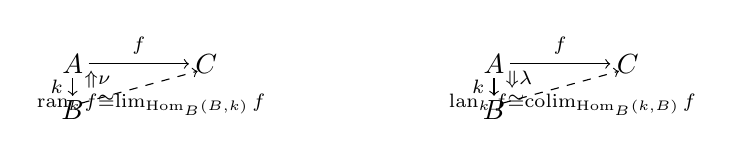
\begin{tikzpicture}[x=1.05em,y=1.05em]
  \begin{scope}
    \node at (0,1.6)   {$A$};
    \node at (4.6,1.6) {$C$};
    \node at (0,0)     {$B$};
    \draw[->] (0.55,1.6) -- node[above]{$\scriptstyle f$} (4.0,1.6);
    \draw[->] (0,1.1)   -- node[left]{$\scriptstyle k$} (0,0.5);
    \draw[->,dashed] (0.3,0.25) -- node[below,pos=0.6]{$\scriptstyle\ran_{k}f\cong\lim_{\HomB(B,k)}f$} (4.3,1.35);
    \node at (0.85,1.05) {$\scriptstyle\Uparrow\nu$};
  \end{scope}
  \qquad
  \begin{scope}[shift={(14.5,0)}]
    \node at (0,1.6)   {$A$};
    \node at (4.6,1.6) {$C$};
    \node at (0,0)     {$B$};
    \draw[->] (0.55,1.6) -- node[above]{$\scriptstyle f$} (4.0,1.6);
    \draw[->] (0,1.1)   -- node[left]{$\scriptstyle k$} (0,0.5);
    \draw[->,dashed] (0.3,0.25) -- node[below,pos=0.6]{$\scriptstyle\lan_{k}f\cong\colim_{\HomB(k,B)}f$} (4.3,1.35);
    \node at (0.85,1.05) {$\scriptstyle\Downarrow\lambda$};
  \end{scope}
\end{tikzpicture}
\end{center}
\end{lemma}

\begin{proof}
由定理 9.3.3(iii)，一个逐点右\trExtension{}定义诸模的一个右\trExtension{}，而一个逐点
左\trExtension{}定义诸模的一个右\trLifting{}：
\begin{center}
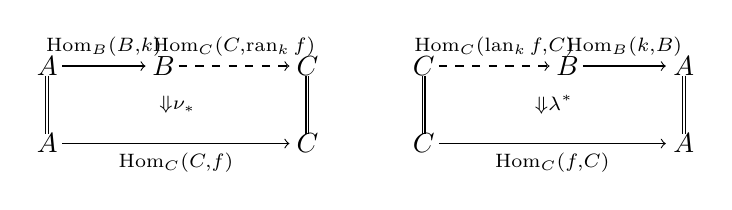
\begin{tikzpicture}[x=1.0em,y=1.0em]
  \begin{scope}
    \node at (0,1.4)   {$A$};
    \node at (4.2,1.4) {$B$};
    \node at (9.4,1.4) {$C$};
    \draw[->] (0.55,1.4) -- node[above]{$\scriptstyle\HomB(B,k)$} (3.55,1.4);
    \draw[->,dashed] (4.75,1.4) -- node[above]{$\scriptstyle\HomC(C,\ran_{k}f)$} (8.75,1.4);
    \draw[double,double distance=0.6pt] (0,1.05) -- (0,-1.05);
    \draw[double,double distance=0.6pt] (9.4,1.05) -- (9.4,-1.05);
    \node at (4.7,0) {$\scriptstyle\Downarrow\nu_{*}$};
    \node at (0,-1.4)   {$A$};
    \node at (9.4,-1.4) {$C$};
    \draw[->] (0.55,-1.4) -- node[below]{$\scriptstyle\HomC(C,f)$} (8.75,-1.4);
  \end{scope}
  \qquad
  \begin{scope}[shift={(13.6,0)}]
    \node at (0,1.4)   {$C$};
    \node at (5.2,1.4) {$B$};
    \node at (9.4,1.4) {$A$};
    \draw[->,dashed] (0.55,1.4) -- node[above]{$\scriptstyle\HomC(\lan_{k}f,C)$} (4.55,1.4);
    \draw[->] (5.75,1.4) -- node[above]{$\scriptstyle\HomB(k,B)$} (8.75,1.4);
    \draw[double,double distance=0.6pt] (0,1.05) -- (0,-1.05);
    \draw[double,double distance=0.6pt] (9.4,1.05) -- (9.4,-1.05);
    \node at (4.7,0) {$\scriptstyle\Downarrow\lambda^{*}$};
    \node at (0,-1.4)   {$C$};
    \node at (9.4,-1.4) {$A$};
    \draw[->] (0.55,-1.4) -- node[below]{$\scriptstyle\HomC(f,C)$} (8.75,-1.4);
  \end{scope}
\end{tikzpicture}
\end{center}
由\cref{def:weighted-limits-colimits}，于是 $\ran_{k}f\cong\lim_{\HomB(B,k)}f$ 且
$\lan_{k}f\cong\colim_{\HomB(k,B)}f$，如所论断。
\end{proof}

在\trEnrichedCategory{}理论中，带\trRepresentable{}权的诸\trWeightedLimit{}或%
\trWeightedColimit{}是通过在表示它们的对象处求值来计算的（见定义 A.6.1）。由类比：

\begin{lemma}\label{lem:representable-weight-restriction}
对任何\trFunctor{} $f\colon A\to C$ 与任何\trGeneralizedElement{} $a\colon X\to A$，
限制 $fa\colon X\to C$ 是 $f$ 由 $A\xrightarrow{\HomA(a,A)}X$ 加权的\trLimit{}，并且
也是 $f$ 由 $X\xrightarrow{\HomA(A,a)}A$ 加权的\trColimit{}。
\end{lemma}

\begin{proof}
由引理 9.1.4，模 $A\xrightarrow{\HomC(C,f)}C$ 沿 $A\xrightarrow{\HomA(a,A)}X$ 的右%
\trExtension{}由 $X\xrightarrow{\HomC(C,fa)}C$ 给出，而模 $C\xrightarrow{\HomC(f,C)}A$
穿过 $X\xrightarrow{\HomA(A,a)}A$ 的右\trLifting{}由 $C\xrightarrow{\HomC(fa,C)}X$
给出。
\begin{center}
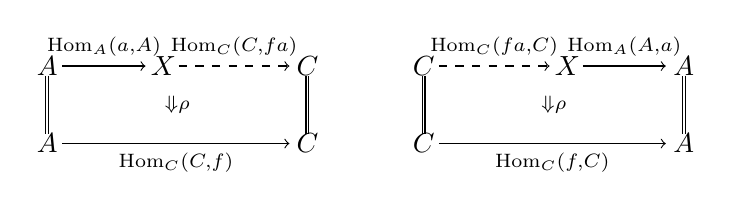
\begin{tikzpicture}[x=1.0em,y=1.0em]
  \begin{scope}
    \node at (0,1.4)   {$A$};
    \node at (4.2,1.4) {$X$};
    \node at (9.4,1.4) {$C$};
    \draw[->] (0.55,1.4) -- node[above]{$\scriptstyle\HomA(a,A)$} (3.55,1.4);
    \draw[->,dashed] (4.75,1.4) -- node[above]{$\scriptstyle\HomC(C,fa)$} (8.75,1.4);
    \draw[double,double distance=0.6pt] (0,1.05) -- (0,-1.05);
    \draw[double,double distance=0.6pt] (9.4,1.05) -- (9.4,-1.05);
    \node at (4.7,0) {$\scriptstyle\Downarrow\rho$};
    \node at (0,-1.4)   {$A$};
    \node at (9.4,-1.4) {$C$};
    \draw[->] (0.55,-1.4) -- node[below]{$\scriptstyle\HomC(C,f)$} (8.75,-1.4);
  \end{scope}
  \qquad
  \begin{scope}[shift={(13.6,0)}]
    \node at (0,1.4)   {$C$};
    \node at (5.2,1.4) {$X$};
    \node at (9.4,1.4) {$A$};
    \draw[->,dashed] (0.55,1.4) -- node[above]{$\scriptstyle\HomC(fa,C)$} (4.55,1.4);
    \draw[->] (5.75,1.4) -- node[above]{$\scriptstyle\HomA(A,a)$} (8.75,1.4);
    \draw[double,double distance=0.6pt] (0,1.05) -- (0,-1.05);
    \draw[double,double distance=0.6pt] (9.4,1.05) -- (9.4,-1.05);
    \node at (4.7,0) {$\scriptstyle\Downarrow\rho$};
    \node at (0,-1.4)   {$C$};
    \node at (9.4,-1.4) {$A$};
    \draw[->] (0.55,-1.4) -- node[below]{$\scriptstyle\HomC(f,C)$} (8.75,-1.4);
  \end{scope}
\end{tikzpicture}
\end{center}
在\cref{def:weighted-limits-colimits}引入的术语之下，这说明：复合函子
$fa\colon X\to C$ 是 $f$ 由表示 $a$ 的那支反变模加权的\trLimit{}，并且也是 $f$ 由表示
$a$ 的那支共变模加权的\trColimit{}。
\end{proof}

由命题 9.1.6及其对偶，我们立即得到：

\begin{proposition}\label{prop:weighted-limits-composite-weights}
对任何\trFunctor{} $f\colon A\to E$ 与 $g\colon C\to E$，以及权 $A\xrightarrow{W}B$
与 $B\xrightarrow{V}C$，诸函子 $\lim_{W\otimes V}f$ 与 $\lim_{W}(\lim_{V}f)$
\trIsomorphism{}，且诸函子 $\colim_{W\otimes V}g$ 与 $\colim_{W}(\colim_{V}g)$
\trIsomorphism{}，只要复合权与这些\trWeightedLimit{}和\trWeightedColimit{}存在。
\end{proposition}

我们由这一结果导出计算\trWeightedLimit{}与\trWeightedColimit{}的若干公式。其中的第一个决定了
一个\trWeightedLimit{}或\trWeightedColimit{}函子在其定义域的\trGeneralizedElement{}处所取的
值。

\begin{lemma}\label{lem:weighted-limit-generalized-element}
若 $f\colon A\to C$ 容许一个由 $A\xrightarrow{W}B$ 加权的\trLimit{}
$\lim_{W}f\colon B\to C$，则对任何\trGeneralizedElement{} $b\colon X\to B$，函子
$\lim_{W}f\circ b\colon X\to C$ \trIsomorphism{}于 $f$ 由 $A\xrightarrow{W(b,1)}X$
加权的\trLimit{}。对偶地，若 $g\colon B\to C$ 容许一个由 $W$ 加权的\trColimit{}
$\colim_{W}g\colon A\to C$，则对任何\trGeneralizedElement{} $a\colon Y\to A$，函子
$\colim_{W}g\circ a\colon Y\to C$ \trIsomorphism{}于 $g$ 由 $Y\xrightarrow{W(1,a)}B$
加权的\trColimit{}。\footnote{原书印作「$\colim_{W}g\circ A$」，按型算（广义
元素 $a\colon Y\to A$，与前句 $b\colon X\to B$ 对称）疑为「$a$」之误，此处径改。
——译者注}
\end{lemma}

\begin{proof}
回忆第 8 章中的命题 8.4.7：$W(b,1)\cong W\otimes\HomB(b,B)$。于是，由%
\cref{prop:weighted-limits-composite-weights}，$f$ 的 $W(b,1)$-\trWeightedLimit{}（若
它存在）是这样一个函子：它右表示模 $\HomC(C,\lim_{W}f)$ 沿模 $\HomB(b,B)$ 的右%
\trExtension{}。由\cref{lem:representable-weight-restriction}，模 $\HomC(C,\lim_{W}f)$
沿 $\HomB(b,B)$ 的右\trExtension{}是模 $\HomC(C,\lim_{W}f\circ b)$。由%
\cref{def:weighted-limits-colimits}，由此可得：$\lim_{W}f\circ b\colon X\to C$ 定义
$f\colon A\to C$ 的 $W(b,1)$-\trWeightedLimit，如所论断。
\end{proof}

第二个有用的计算性结果把一般的\trWeightedLimit{}或\trWeightedColimit{}约化为\trHomotopyTwoCategory{}中
的右\trExtension{}或左\trExtension{}。

\begin{lemma}\label{lem:weights-as-pointwise-extensions}
考虑由双侧\trTwoSidedIsofibration{}
$A\overset{q}{\twoheadleftarrow}W\overset{p}{\twoheadrightarrow}B$ 所编码的一支权
$A\xrightarrow{W}B$。

（i）对任何\trFunctor{} $f\colon A\to C$，\trWeightedLimit{}
$\lim_{W}f\colon B\to C$ 由逐点右\trExtension
\begin{center}
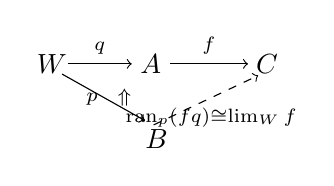
\begin{tikzpicture}[x=1.05em,y=1.05em]
  \node at (0,1.6)   {$W$};
  \node at (3.4,1.6) {$A$};
  \node at (7.4,1.6) {$C$};
  \draw[->] (0.55,1.6) -- node[above]{$\scriptstyle q$} (2.75,1.6);
  \draw[->] (4.05,1.6) -- node[above]{$\scriptstyle f$} (6.75,1.6);
  \draw[->] (0.35,1.25) -- node[left,pos=0.55]{$\scriptstyle p$} (3.2,-0.35);
  \draw[->,dashed] (3.5,-0.5) -- node[below,pos=0.55]{$\scriptstyle\ran_{p}(fq)\cong\lim_{W}f$} (7.1,1.2);
  \node at (2.5,0.45) {$\scriptstyle\Uparrow$};
  \node at (3.6,-1.0) {$B$};
\end{tikzpicture}
\end{center}
给出。

（ii）对任何\trFunctor{} $g\colon B\to C$，\trWeightedColimit{} $\colim_{W}g\colon A\to C$ 由
逐点左\trExtension
\begin{center}
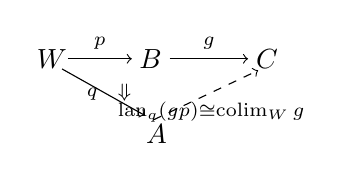
\begin{tikzpicture}[x=1.05em,y=1.05em]
  \node at (0,1.6)   {$W$};
  \node at (3.4,1.6) {$B$};
  \node at (7.4,1.6) {$C$};
  \draw[->] (0.55,1.6) -- node[above]{$\scriptstyle p$} (2.75,1.6);
  \draw[->] (4.05,1.6) -- node[above]{$\scriptstyle g$} (6.75,1.6);
  \draw[->] (0.35,1.25) -- node[left,pos=0.55]{$\scriptstyle q$} (3.2,-0.35);
  \draw[->,dashed] (3.5,-0.5) -- node[below,pos=0.55]{$\scriptstyle\lan_{q}(gp)\cong\colim_{W}g$} (7.1,1.2);
  \node at (2.5,0.45) {$\scriptstyle\Downarrow$};
  \node at (3.6,-1.0) {$A$};
\end{tikzpicture}
\end{center}
给出。\footnote{原书此虚线标签印作「$\lan_{q}(fp)\cong\colim_{W}f$」，两处 $f$
均疑为（ii）款所设之 $g$ 之误（（i）款相应式为 $\ran_{p}(fq)\cong\lim_{W}f$），
此处径改。——译者注}

特别地，由从 $A$ 到 $1$ 的模加权的诸\trLimit{}与由从 $1$ 到 $B$ 的模加权的诸%
\trColimit{}约化为普通的\trLimit{}与\trColimit{}。
\end{lemma}

\begin{proof}
回忆第 8 章中的命题 8.3.11：任何模
$A\overset{q}{\twoheadleftarrow}W\overset{p}{\twoheadrightarrow}B$ 都分解为一个复合
$\HomA(q,A)\otimes\HomB(B,p)\simeq W$。于是由%
\cref{prop:weighted-limits-composite-weights}、%
\cref{lem:weighted-limit-generalized-element}与\cref{lem:pointwise-extensions-weighted}
\begin{equation*}
\lim_{W}f\cong\lim_{\HomB(B,p)}\bigl(\lim_{\HomA(q,A)}f\bigr)\cong
\lim_{\HomB(B,p)}(fq)\cong\ran_{p}(fq).
\end{equation*}
\end{proof}

在一个\trCartesianClosed{}\trInfinityCosmos{}中，第 2 章中的定理 2.4.2 证明了：右
伴随保持以∞-范畴为指标的图表的\trLimit{}，而左伴随保持其\trColimit。现在我们可以把这个
结果推广到\trWeightedLimit{}与\trWeightedColimit{}，同时舍去外围\trInfinityCosmos{}是%
\trCartesianClosed{}这一假设。

\begin{theorem}\label{thm:adjoints-preserve-weighted-limits}
\trRightAdjoint{}保持\trWeightedLimit{}，而\trLeftAdjoint{}保持\trWeightedColimit{}。
\end{theorem}

\begin{proof}
考虑一支权 $J\xrightarrow{W}K$、一个\trDiagram{} $d\colon J\to A$，以及一个%
\trAdjunction{}，其\trRightAdjoint{}为 $u\colon A\to B$ 而\trLeftAdjoint{}为
$f\colon B\to A$。\trWeightedLimit{} $\lim_{W}d\colon K\to A$ 定义了诸模的一个右%
\trExtension
\begin{center}
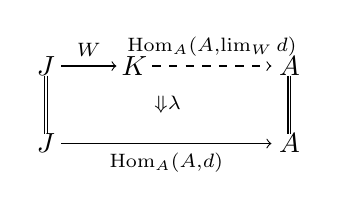
\begin{tikzpicture}[x=1.0em,y=1.0em]
  \node at (0,1.4)   {$J$};
  \node at (3.2,1.4) {$K$};
  \node at (8.8,1.4) {$A$};
  \draw[->] (0.55,1.4) -- node[above]{$\scriptstyle W$} (2.55,1.4);
  \draw[->,dashed] (3.85,1.4) -- node[above]{$\scriptstyle\HomA(A,\lim_{W}d)$} (8.15,1.4);
  \draw[double,double distance=0.6pt] (0,1.05) -- (0,-1.05);
  \draw[double,double distance=0.6pt] (8.8,1.05) -- (8.8,-1.05);
  \node at (4.4,0) {$\scriptstyle\Downarrow\lambda$};
  \node at (0,-1.4)   {$J$};
  \node at (8.8,-1.4) {$A$};
  \draw[->] (0.55,-1.4) -- node[below]{$\scriptstyle\HomA(A,d)$} (8.15,-1.4);
\end{tikzpicture}
\end{center}
我们的任务是证明：由下左方的胞腔穿过下右方的复合的唯一因子分解所定义的胞腔 $u\lambda$
仍是诸模的一个右\trExtension{}：
\begin{center}
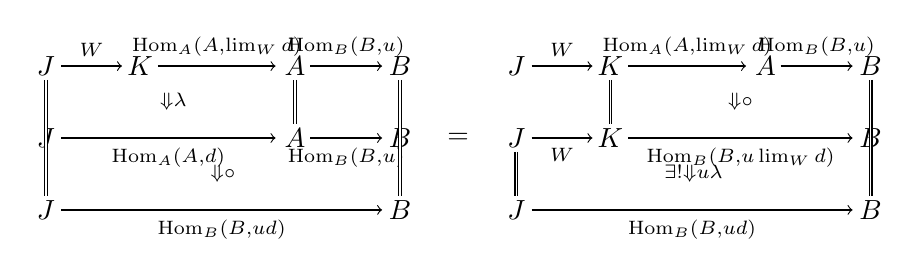
\begin{tikzpicture}[x=1.0em,y=1.0em]
  \begin{scope}
    \node at (0,2.6)    {$J$};
    \node at (3.4,2.6)  {$K$};
    \node at (9.0,2.6)  {$A$};
    \node at (12.8,2.6) {$B$};
    \draw[->] (0.55,2.6) -- node[above]{$\scriptstyle W$} (2.75,2.6);
    \draw[->] (4.05,2.6) -- node[above]{$\scriptstyle\HomA(A,\lim_{W}d)$} (8.3,2.6);
    \draw[->] (9.55,2.6) -- node[above]{$\scriptstyle\HomB(B,u)$} (12.15,2.6);
    \node at (0,0)    {$J$};
    \node at (9.0,0)  {$A$};
    \node at (12.8,0) {$B$};
    \draw[->] (0.55,0) -- node[below]{$\scriptstyle\HomA(A,d)$} (8.3,0);
    \draw[->] (9.55,0) -- node[below]{$\scriptstyle\HomB(B,u)$} (12.15,0);
    \node at (0,-2.6)    {$J$};
    \node at (12.8,-2.6) {$B$};
    \draw[->] (0.55,-2.6) -- node[below]{$\scriptstyle\HomB(B,ud)$} (12.15,-2.6);
    \draw[double,double distance=0.6pt] (0,2.1) -- (0,-2.1);
    \draw[double,double distance=0.6pt] (9.0,2.1) -- (9.0,0.5);
    \draw[double,double distance=0.6pt] (12.8,2.1) -- (12.8,-2.1);
    \node at (4.6,1.3)  {$\scriptstyle\Downarrow\lambda$};
    \node at (6.4,-1.3) {$\scriptstyle\Downarrow\circ$};
  \end{scope}
  \node at (14.9,0) {$=$};
  \begin{scope}[shift={(17.0,0)}]
    \node at (0,2.6)    {$J$};
    \node at (3.4,2.6)  {$K$};
    \node at (9.0,2.6)  {$A$};
    \node at (12.8,2.6) {$B$};
    \draw[->] (0.55,2.6) -- node[above]{$\scriptstyle W$} (2.75,2.6);
    \draw[->] (4.05,2.6) -- node[above]{$\scriptstyle\HomA(A,\lim_{W}d)$} (8.3,2.6);
    \draw[->] (9.55,2.6) -- node[above]{$\scriptstyle\HomB(B,u)$} (12.15,2.6);
    \node at (0,0)    {$J$};
    \node at (3.4,0)  {$K$};
    \node at (12.8,0) {$B$};
    \draw[->] (0.55,0) -- node[below]{$\scriptstyle W$} (2.75,0);
    \draw[->] (4.05,0) -- node[below]{$\scriptstyle\HomB(B,u\lim_{W}d)$} (12.15,0);
    \node at (0,-2.6)    {$J$};
    \node at (12.8,-2.6) {$B$};
    \draw[->] (0.55,-2.6) -- node[below]{$\scriptstyle\HomB(B,ud)$} (12.15,-2.6);
    \draw[double,double distance=0.6pt] (0,-0.5) -- (0,-2.1);
    \draw[double,double distance=0.6pt] (3.4,2.1) -- (3.4,0.5);
    \draw[double,double distance=0.6pt] (12.8,2.1) -- (12.8,-2.1);
    \node at (8.1,1.3)  {$\scriptstyle\Downarrow\circ$};
    \node at (6.4,-1.3) {$\scriptstyle\exists!\Downarrow u\lambda$};
  \end{scope}
\end{tikzpicture}
\end{center}
为此，考虑一个胞腔
\begin{center}
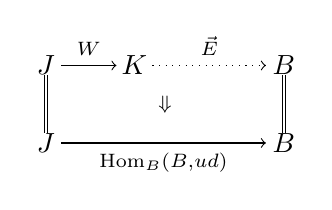
\begin{tikzpicture}[x=1.0em,y=1.0em]
  \node at (0,1.4)   {$J$};
  \node at (3.2,1.4) {$K$};
  \node at (8.6,1.4) {$B$};
  \draw[->] (0.55,1.4) -- node[above]{$\scriptstyle W$} (2.55,1.4);
  \draw[->,dotted] (3.85,1.4) -- node[above]{$\scriptstyle\vec{E}$} (7.95,1.4);
  \draw[double,double distance=0.6pt] (0,1.05) -- (0,-1.05);
  \draw[double,double distance=0.6pt] (8.6,1.05) -- (8.6,-1.05);
  \node at (4.3,0) {$\scriptstyle\Downarrow$};
  \node at (0,-1.4)   {$J$};
  \node at (8.6,-1.4) {$B$};
  \draw[->] (0.55,-1.4) -- node[below]{$\scriptstyle\HomB(B,ud)$} (7.95,-1.4);
\end{tikzpicture}
\end{center}
由第 4 章中的推论 4.1.3，存在一个\trEquivalence{} $\HomB(B,ud)\simeq\HomA(f,d)$，从而
由第 8 章中的命题 8.2.1，存在一个限制胞腔
\begin{center}
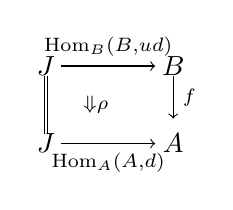
\begin{tikzpicture}[x=1.0em,y=1.0em]
  \node at (0,1.4)  {$J$};
  \node at (4.6,1.4){$B$};
  \draw[->] (0.55,1.4) -- node[above]{$\scriptstyle\HomB(B,ud)$} (3.95,1.4);
  \draw[double,double distance=0.6pt] (0,1.05) -- (0,-1.05);
  \node at (1.8,0) {$\scriptstyle\Downarrow\rho$};
  \draw[->] (4.6,1.05) -- node[right]{$\scriptstyle f$} (4.6,-0.5);
  \node at (0,-1.4)  {$J$};
  \node at (4.6,-1.4){$A$};
  \draw[->] (0.55,-1.4) -- node[below]{$\scriptstyle\HomA(A,d)$} (3.95,-1.4);
\end{tikzpicture}
\end{center}

使得与 $\rho$ 的复合在形如 $W\divideontimes\vec{E}\Rightarrow\HomB(B,ud)$ 的诸胞腔与下左方
所示形状的诸胞腔之间诱导一个双射：
\begin{center}
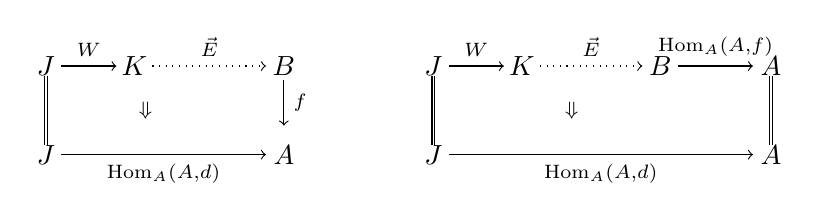
\begin{tikzpicture}[x=1.0em,y=1.0em]
  \begin{scope}
    \node at (0,1.6)   {$J$};
    \node at (3.2,1.6) {$K$};
    \node at (8.6,1.6) {$B$};
    \draw[->] (0.55,1.6) -- node[above]{$\scriptstyle W$} (2.55,1.6);
    \draw[->,dotted] (3.85,1.6) -- node[above]{$\scriptstyle\vec{E}$} (7.95,1.6);
    \draw[->] (8.6,1.1) -- node[right]{$\scriptstyle f$} (8.6,-0.55);
    \draw[double,double distance=0.6pt] (0,1.25) -- (0,-1.25);
    \node at (3.6,0) {$\scriptstyle\Downarrow$};
    \node at (0,-1.6)   {$J$};
    \node at (8.6,-1.6) {$A$};
    \draw[->] (0.55,-1.6) -- node[below]{$\scriptstyle\HomA(A,d)$} (7.95,-1.6);
  \end{scope}
  \node at (11.4,0) {$\leftrightsquigarrow$};
  \begin{scope}[shift={(14.0,0)}]
    \node at (0,1.6)    {$J$};
    \node at (3.2,1.6)  {$K$};
    \node at (8.2,1.6)  {$B$};
    \node at (12.2,1.6) {$A$};
    \draw[->] (0.55,1.6) -- node[above]{$\scriptstyle W$} (2.55,1.6);
    \draw[->,dotted] (3.85,1.6) -- node[above]{$\scriptstyle\vec{E}$} (7.55,1.6);
    \draw[->] (8.85,1.6) -- node[above]{$\scriptstyle\HomA(A,f)$} (11.55,1.6);
    \draw[double,double distance=0.6pt] (0,1.25) -- (0,-1.25);
    \draw[double,double distance=0.6pt] (12.2,1.25) -- (12.2,-1.25);
    \node at (5.0,0) {$\scriptstyle\Downarrow$};
    \node at (0,-1.6)    {$J$};
    \node at (12.2,-1.6) {$A$};
    \draw[->] (0.55,-1.6) -- node[below]{$\scriptstyle\HomA(A,d)$} (11.55,-1.6);
  \end{scope}
\end{tikzpicture}
\end{center}
由第 8 章中的定理 8.4.4，这些胞腔与上右方所示形状的诸胞腔处于一个自然双射之中。由于
$\HomA(A,\lim_{W}d)$ 是 $\HomA(A,d)$ 沿 $W$ 的一个右\trExtension{}，这类胞腔与下左方
所示形状的诸胞腔处于双射之中
\begin{center}
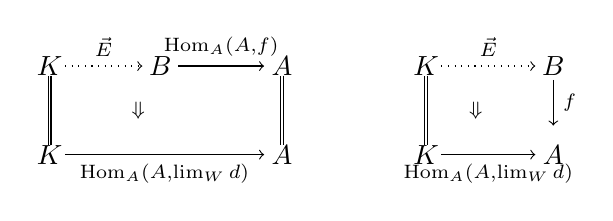
\begin{tikzpicture}[x=1.0em,y=1.0em]
  \begin{scope}
    \node at (0,1.6)   {$K$};
    \node at (4.0,1.6) {$B$};
    \node at (8.4,1.6) {$A$};
    \draw[->,dotted] (0.55,1.6) -- node[above]{$\scriptstyle\vec{E}$} (3.35,1.6);
    \draw[->] (4.65,1.6) -- node[above]{$\scriptstyle\HomA(A,f)$} (7.75,1.6);
    \draw[double,double distance=0.6pt] (0,1.25) -- (0,-1.25);
    \draw[double,double distance=0.6pt] (8.4,1.25) -- (8.4,-1.25);
    \node at (3.2,0) {$\scriptstyle\Downarrow$};
    \node at (0,-1.6)   {$K$};
    \node at (8.4,-1.6) {$A$};
    \draw[->] (0.55,-1.6) -- node[below]{$\scriptstyle\HomA(A,\lim_{W}d)$} (7.75,-1.6);
  \end{scope}
  \node at (11.0,0) {$\leftrightsquigarrow$};
  \begin{scope}[shift={(13.6,0)}]
    \node at (0,1.6)   {$K$};
    \node at (4.6,1.6) {$B$};
    \draw[->,dotted] (0.55,1.6) -- node[above]{$\scriptstyle\vec{E}$} (3.95,1.6);
    \draw[->] (4.6,1.1) -- node[right]{$\scriptstyle f$} (4.6,-0.55);
    \draw[double,double distance=0.6pt] (0,1.25) -- (0,-1.25);
    \node at (1.8,0) {$\scriptstyle\Downarrow$};
    \node at (0,-1.6)   {$K$};
    \node at (4.6,-1.6) {$A$};
    \draw[->] (0.55,-1.6) -- node[below]{$\scriptstyle\HomA(A,\lim_{W}d)$} (3.95,-1.6);
  \end{scope}
\end{tikzpicture}
\end{center}
而再次由第 8 章中的定理 8.4.4，这些胞腔与上右方所示形状的诸胞腔处于一个自然双射之中。
由第 8 章中的命题 8.2.1，这类胞腔与通过沿 $f\colon B\to A$ 的限制 $\HomA(f,\lim_{W}d)$
（即 $\HomA(A,\lim_{W}d)$ 沿 $f$ 的限制）作因子分解所定义的诸胞腔处于双射之中。由
第 4 章中的推论 4.1.3，存在模的一个\trEquivalence{}
$\HomA(f,\lim_{W}d)\simeq\HomB(B,u\lim_{W}d)$，于是经由这一限制，这些胞腔双射于如下
形状的诸胞腔
\begin{center}
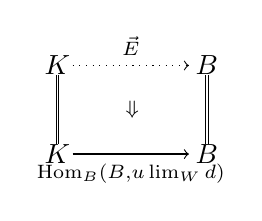
\begin{tikzpicture}[x=1.0em,y=1.0em]
  \node at (0,1.6)   {$K$};
  \node at (5.4,1.6) {$B$};
  \draw[->,dotted] (0.55,1.6) -- node[above]{$\scriptstyle\vec{E}$} (4.75,1.6);
  \draw[double,double distance=0.6pt] (0,1.25) -- (0,-1.25);
  \draw[double,double distance=0.6pt] (5.4,1.25) -- (5.4,-1.25);
  \node at (2.7,0) {$\scriptstyle\Downarrow$};
  \node at (0,-1.6)   {$K$};
  \node at (5.4,-1.6) {$B$};
  \draw[->] (0.55,-1.6) -- node[below]{$\scriptstyle\HomB(B,u\lim_{W}d)$} (4.75,-1.6);
\end{tikzpicture}
\end{center}
当我们从模 $\HomB(B,u\lim_{W}d)$ 处的恒同胞腔出发实施这一双射、再反转这个复合双射
时，便得到胞腔
$u\lambda\colon W\divideontimes\HomB(B,u\lim_{W}d)\Rightarrow\HomB(B,ud)$；这就证明了
$u\lambda$ 把 $\HomB(B,u\lim_{W}d)$ 显示为 $\HomB(B,ud)$ 沿 $W$ 的右\trExtension{}。
于是 $u\lim_{W}d$ 是 $ud$ 的 $W$-\trWeightedLimit{}，如所论断。
\end{proof}

\cref{thm:adjoints-preserve-weighted-limits}应当与命题 A.6.20 相比较，后者观察到：
富集范畴论的诸右伴随保持 A.6 节中所定义的\trWeightedLimit{}。在 $(\infty,1)$-范畴的%
\trInfinityCosmos{}中，我们可以把本节的结果视为在为弱富集于\trInfinityGroupoid{}之
上的诸范畴发展一门类似的\trWeightedLimit{}与\trWeightedColimit{}理论。特别地，$(\infty,1)$-
范畴之间的诸\trAdjunction{}自动地富集于\trInfinityGroupoid{}之上（如第 4 章中的
注 4.1.4 所暗示的那样），因此应当预期它们保持由\trFiber{}为\trInfinityGroupoid{}的
那些\trModule{}所加权的极限。

\subsection*{练习}

\begin{exercise}\label{ex:ordinary-limits-as-weighted}
确定诸权 $W_{\mathrm{lim}}$ 与 $W_{\mathrm{colim}}$，使得一个\trDiagram{} $f$ 的
$W_{\mathrm{lim}}$-\trWeightedLimit{}是 $f$ 的普通\trLimit{}（如定义 9.4.7 中所定义
的那样），而 $W_{\mathrm{colim}}$-\trWeightedColimit{}是普通\trColimit{}。
\end{exercise}

\begin{exercise}\label{ex:tensor-cotensor-as-weighted}
将一个\trInfinityCategory{}的\trElement{} $a\colon 1\to A$ 由一个\trDiscrete{}%
\trInfinityCategory{} $S$ 所取的\textbf{\trTensor}与\textbf{\trCotensor}分别定义为
一个\trWeightedColimit{}与一个\trWeightedLimit{}，并把这一构造与第 4 章中的定义 4.3.6 相比较。
\end{exercise}


